% Board power measurement procedure for the ZedBoard super-resolution designs.
% Build: pdflatex power_procedure.tex (twice).
\documentclass[11pt,a4paper]{article}
\usepackage[T1]{fontenc}
\usepackage[utf8]{inputenc}
\usepackage{lmodern}
\usepackage[a4paper,margin=20mm]{geometry}
\usepackage{booktabs,tabularx,array,longtable}
\usepackage{enumitem}
\usepackage{xcolor}
\usepackage{tikz}
\usetikzlibrary{arrows.meta,positioning,calc}
\usepackage{listings}
\usepackage{fancyhdr}
\usepackage[hidelinks]{hyperref}
\usepackage{amsmath,amssymb}
\def\UrlBreaks{\do\/\do-\do_\do.}
\setlist{itemsep=2pt,topsep=3pt}
\setlength{\parindent}{0pt}
\setlength{\parskip}{5pt}
\newcolumntype{L}{>{\raggedright\arraybackslash}X}
\definecolor{warn}{HTML}{B91C1C}
\definecolor{boxbg}{HTML}{F3F4F6}
\lstset{basicstyle=\ttfamily\footnotesize,breaklines=true,columns=fullflexible,keepspaces=true,
  frame=single,backgroundcolor=\color{boxbg},rulecolor=\color{black!30},xleftmargin=2pt,xrightmargin=2pt}
\newcommand{\warnbox}[1]{\par\noindent\fcolorbox{warn}{warn!6}{\parbox{\dimexpr\linewidth-2\fboxsep-2\fboxrule}{\textbf{\color{warn}Warning.} #1}}\par}
\pagestyle{fancy}\fancyhf{}\fancyhead[L]{\small ZedBoard power measurement procedure}\fancyhead[R]{\small 11 Nov 2026}\fancyfoot[C]{\small\thepage}

\begin{document}

\begin{center}
{\LARGE\bfseries Measuring the Board Power of the\\[2pt] Super-Resolution Accelerator on the ZedBoard}\\[6pt]
{\large Step-by-step procedure for R0, the pipeline and pipeline v2 packed}\\[4pt]
{\small Prepared 11 November 2026. Nothing in this document has been run on the board yet.}
\end{center}

\section*{Contents at a glance}
\begin{enumerate}[label=\arabic*.]
  \item What is measured and why (page~\pageref{sec:what})
  \item Is your equipment suitable? (page~\pageref{sec:equip})
  \item Where to connect on the ZedBoard (page~\pageref{sec:where})
  \item Setting up the bench supply and the meters (page~\pageref{sec:setup})
  \item The measurement states and the exact commands (page~\pageref{sec:states})
  \item How to take the readings (page~\pageref{sec:read})
  \item Calculations (page~\pageref{sec:calc})
  \item Recording sheet (page~\pageref{sec:sheet})
  \item What to send back and how to report it in the paper (page~\pageref{sec:report})
\end{enumerate}

%==========================================================================
\section{What is measured and why}\label{sec:what}

All power numbers in the report and the paper are so far \textbf{Vivado estimates} of the Zynq chip only (1.913\,W for R0, 2.290\,W for the pipeline, 2.51\,W for pipeline v2 packed, confidence ``Low''). Reviewers will ask for a measurement. The measurement below gives:

\begin{itemize}
  \item the \textbf{board input power} $P = V_\mathrm{in}\times I_\mathrm{in}$ at the 12\,V input of the ZedBoard, in each state (board on, design loaded but idle, design processing);
  \item the \textbf{accelerator power above idle}, $P_2 - P_1$, which is the useful number for comparing designs, because the board overhead (DDR, regulators, USB-UART, LEDs) is the same in every state;
  \item the \textbf{energy per frame} and \textbf{frames per second per watt}, the numbers that can be compared with Liu et al.\ 2024 (2.12\,fps/W at 16.85\,W board power, measured with a power meter).
\end{itemize}

This is \textbf{board-level} power (the whole ZedBoard), not chip power. It must never be put in the same row as the Vivado on-chip estimate without saying so.

%==========================================================================
\section{Is your equipment suitable?}\label{sec:equip}

\begin{tabularx}{\textwidth}{@{}p{0.28\textwidth}p{0.12\textwidth}L@{}}
\toprule
\textbf{Instrument} & \textbf{Use it?} & \textbf{How} \\ \midrule
DC power supply & \textbf{Yes, as the 12\,V source} & Replaces the 12\,V wall adapter. It gives an exact, stable 12.00\,V, and its current display gives a first current reading. Use only its \emph{DC output}; do not use the waveform/function-generator output for the board. \\
Digital multimeter & \textbf{Yes} & (a) In \emph{DC mV} mode across header J21 (current-sense resistor); (b) in \emph{DC V} mode at the board input to read $V_\mathrm{in}$; (c) optionally in series as an ammeter on its high-current range (1\,A or more, never the 200/400\,mA range). \\
Oscilloscope & \textbf{Not needed} & The changes are slow (seconds), so a meter is enough. Do \textbf{not} connect the scope ground clip to J21: one side of J21 is at +12\,V, and the scope ground is connected to mains earth, so the clip can short the 12\,V supply (see the warning in Section~\ref{sec:where}). \\
\bottomrule
\end{tabularx}

\medskip
If you have a second multimeter, use one across J21 (current) and one at the input (voltage) at the same time; otherwise read them one after the other in the same 30\,s window.

\textbf{Resolution decides which reading is the primary one.} The board draws a few hundred mA at 12\,V, and the differences between states are only tens of mA. Before starting, write down the resolution of each instrument and use the one with the finest current resolution as the primary reading:

\begin{tabularx}{\textwidth}{@{}lccL@{}}
\toprule
\textbf{Reading} & \textbf{Resolution} & \textbf{= current step} & \textbf{= power step at 12\,V} \\ \midrule
Supply display, 10\,mA steps & 10\,mA & 10\,mA & 120\,mW (too coarse for deltas) \\
Supply display, 1\,mA steps & 1\,mA & 1\,mA & 12\,mW (good) \\
Multimeter across J21, 0.1\,mV steps & 0.1\,mV & 10\,mA & 120\,mW (coarse) \\
Multimeter across J21, 0.01\,mV steps & 0.01\,mV & 1\,mA & 12\,mW (good) \\
Multimeter in series, 1\,mA steps & 1\,mA & 1\,mA & 12\,mW (good) \\
\bottomrule
\end{tabularx}

\medskip
Current through J21: $I = V_{J21}/0.010\,\Omega$, so 1\,mV across J21 means 100\,mA.

%==========================================================================
\section{Where to connect on the ZedBoard}\label{sec:where}

The ZedBoard Hardware User's Guide (v2.2) states that a \textbf{10\,m$\Omega$, 1\,W current-sense resistor} is in series with the 12\,V input, and that \textbf{header J21} straddles this resistor so that its voltage can be measured to calculate the board power. (The guide prints the formula as $V^2/R$, which is wrong for power; use $I = V/R$, $P = I\times V_\mathrm{in}$, as the forum threads on this point also explain.)

\textbf{Find these parts on your board} (check the white silkscreen text next to each part; the positions below are the usual ones, but trust the label printed on your board):
\begin{itemize}
  \item \textbf{J20}: the round 12\,V DC barrel jack at the board edge (2.1\,mm plug, \textbf{centre pin positive}).
  \item \textbf{SW8}: the slide power switch next to the barrel jack.
  \item \textbf{J21}: a small 2-pin header near the power input, across the current-sense resistor (R292 on the schematic).
\end{itemize}

\begin{center}
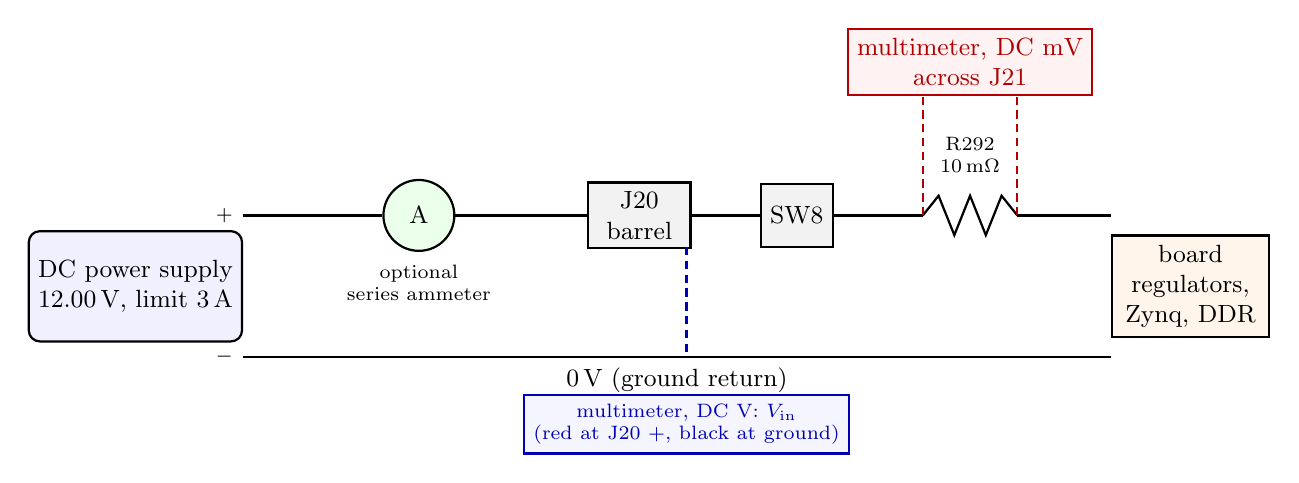
\begin{tikzpicture}[>=Stealth, every node/.style={font=\small}, thick]
  \node[draw, rounded corners, minimum width=26mm, minimum height=14mm, align=center, fill=blue!6] (psu) at (0,0) {DC power supply\\ 12.00\,V, limit 3\,A};
  \node[draw, circle, minimum size=9mm, fill=green!8] (amm) at (3.6,0.9) {A};
  \node[below=1pt of amm, font=\scriptsize, align=center] {optional\\series ammeter};
  \node[draw, minimum width=13mm, minimum height=8mm, align=center, fill=gray!10] (jack) at (6.4,0.9) {J20\\barrel};
  \node[draw, minimum width=9mm, minimum height=8mm, align=center, fill=gray!10] (sw) at (8.4,0.9) {SW8};
  \draw (9.6,0.9) -- (10.0,0.9);
  \draw (10.0,0.9) -- (10.2,1.15) -- (10.4,0.65) -- (10.6,1.15) -- (10.8,0.65) -- (11.0,1.15) -- (11.2,0.9);
  \node[above=6pt, font=\scriptsize, align=center] at (10.6,1.1) {R292\\10\,m$\Omega$};
  \node[draw, minimum width=20mm, minimum height=12mm, align=center, fill=orange!8] (reg) at (13.4,0.0) {board\\regulators,\\Zynq, DDR};
  \draw (psu.east |- 0,0.9) -- (amm.west);
  \draw (amm.east) -- (jack.west);
  \draw (jack.east) -- (sw.west);
  \draw (sw.east) -- (9.6,0.9);
  \draw (11.2,0.9) -- (reg.west |- 0,0.9);
  \draw (psu.east |- 0,-0.9) -- (reg.west |- 0,-0.9) node[midway, below] {0\,V (ground return)};
  \node[left, font=\scriptsize] at (psu.east |- 0,0.9) {$+$};
  \node[left, font=\scriptsize] at (psu.east |- 0,-0.9) {$-$};
  % J21 meter
  \draw[densely dashed, red!70!black] (10.0,0.9) -- (10.0,2.4);
  \draw[densely dashed, red!70!black] (11.2,0.9) -- (11.2,2.4);
  \node[draw, red!70!black, fill=red!5, minimum width=24mm, align=center] at (10.6,2.85) {multimeter, DC mV\\across J21};
  % Vin meter
  \draw[densely dashed, blue!70!black] (7.0,0.5) -- (7.0,-0.9);
  \node[draw, blue!70!black, fill=blue!4, align=center, font=\scriptsize] at (7.0,-1.75) {multimeter, DC V: $V_\mathrm{in}$\\(red at J20 $+$, black at ground)};
\end{tikzpicture}
\end{center}

\warnbox{J21 is on the \emph{high side}: both of its pins are at about +12\,V. A multimeter is floating, so it is safe across J21. The oscilloscope ground clip is \emph{not} floating (it is tied to mains earth). If the supply's negative terminal is also earthed, clipping the scope ground onto J21 shorts the 12\,V supply. Do not use the oscilloscope on J21.}

\warnbox{Never put the multimeter in \emph{current} (A or mA) mode across J21. In current mode the meter is almost a short circuit; across J21 it does no harm to the resistor but measures nothing useful, and on the mA range it can blow the meter's fuse. Across J21 always use the \textbf{DC mV} (voltage) mode.}

%==========================================================================
\section{Setting up the bench supply and the meters}\label{sec:setup}

Do these steps with the board's power switch SW8 \textbf{off}.

\begin{enumerate}
  \item \textbf{Cable.} Use a cable with a 2.1\,mm barrel plug (centre positive), or cut the cable of a spare 12\,V adapter. Connect the plug's centre conductor to the supply's \textbf{$+$} and the outer sleeve to \textbf{$-$}.
  \item \textbf{Set the supply before connecting the board.} Output off; voltage \textbf{12.00\,V}; current limit \textbf{3.0\,A} (the ZedBoard's adapter is rated 12\,V, 3\,A). Turn the output on and check with the multimeter (DC V) at the plug: centre $+12.0$\,V against the sleeve. If it reads $-12$\,V, the polarity is reversed: fix it before going on.
  \item Turn the supply output off, plug the barrel plug into J20.
  \item \textbf{Optional series ammeter:} only if your multimeter has a current range of at least 1\,A with 1\,mA resolution. Break the $+$ wire and insert the meter (red lead to the supply side, black lead to the board side). Never use the 200/400\,mA range: the board can exceed it at switch-on.
  \item \textbf{J21 meter:} multimeter in \textbf{DC mV} mode, leads on the two J21 pins (use small hook clips or header jumper wires so that nothing slips onto other pins). The pin on the supply side is the more positive one; if the meter shows a negative value, just note it as positive (the sign only means the leads are swapped).
  \item \textbf{$V_\mathrm{in}$ meter:} DC V between the J20 centre pin (or the supply side of J21) and a ground point (for example the shield of a USB connector). Measure it at the board, not at the supply: the cable and a series ammeter drop some voltage.
  \item Connect the two USB cables as usual (PROG/JTAG J17 and UART), turn the supply output on, then switch SW8 on. The green power LED must light.
  \item \textbf{Zero check of the J21 meter:} before switching SW8 on, the J21 reading must be 0.00\,mV ($\pm$ the last digit). Note the offset, if any, and subtract it from every reading.
\end{enumerate}

Keep the board in the same place, with the same cables and USB connections, for the whole session, and keep the room temperature steady (no fan pointed at the board halfway through).

%==========================================================================
\section{The measurement states and the exact commands}\label{sec:states}

Every command is run from the main project folder, after loading the Vitis tools. Open a second terminal with the UART (\texttt{picocom -b 115200 /dev/ttyACM0}) to see when processing starts and ends.

\begin{lstlisting}
cd ~/Desktop/venkat/sem_project_all
source ~/Desktop/vivado_install/Vitis/2024.1/settings64.sh
V=~/Desktop/venkat; PS=$V/power_session
LR=data/board/div2k_img0193_lr_960x540.raw
\end{lstlisting}

The folder \texttt{\textasciitilde/Desktop/venkat/power\_session} already contains the 125\,MHz clock set-up files of the pipeline and of pipeline v2 packed, extracted from their XSA files (both md5 \texttt{d2a7789c\ldots}, the same file that was used on the board on 28 Oct and 10 Nov 2026). Every run reads the clock registers back and refuses to start if the PL clock is not the expected one (100 or 125\,MHz).

\subsection*{The states}

\begin{longtable}{@{}p{0.07\textwidth}p{0.27\textwidth}p{0.58\textwidth}@{}}
\toprule
\textbf{State} & \textbf{What runs} & \textbf{Duration of the run (processing part)} \\ \midrule
\endhead
P0 & board on, FPGA not programmed & as long as needed (power on, do nothing) \\
R0-P1 & R0 bitstream, ARM idle & after T1 has finished (idle loop) \\
R0-P2 & R0, 200 frames & about 262\,s (200 $\times$ 1.312\,s) \\
PI-P1 & pipeline bitstream, ARM idle & after T1 has finished \\
PI-P2 & pipeline, 1000 frames, cached buffers & about 95\,s (1000 $\times$ 95.4\,ms) \\
PP-P1 & pipeline v2 packed, ARM idle & after T1 has finished \\
PP-P2c & v2 packed, 1500 frames, cached buffers & about 92\,s (1500 $\times$ 61.6\,ms) \\
PP-P2n & v2 packed, 2500 frames, non-cacheable buffers (the 27.1\,fps build) & about 92\,s (2500 $\times$ 36.95\,ms) \\
P3 & R0 bitstream, ARM only computes (no accelerator) & about 269\,s (20 $\times$ 13.44\,s) \\
R0-P1/P2 again & repeat of R0 at the end & drift check \\
\bottomrule
\end{longtable}

The run times above are the board-measured frame times multiplied by the frame count. Loading the bitstream, the program and the input image over JTAG takes some extra seconds \emph{before} processing starts: start the readings only after the UART prints the line \texttt{T3: timing, N frames} (or \texttt{T7}), plus a few seconds.

\subsection*{Commands}

\textbf{P0.} Switch the board on; do not run anything. Read the meters (Section~\ref{sec:read}).

\textbf{R0 (100\,MHz).}
\begin{lstlisting}
# R0-P1: idle (T1 ends in an idle loop; read the meters after the command has returned)
SR_EXPECT_MHZ=100 xsdb software/board/run_board_clk.tcl software/board/build/sr_app_t1.elf - - $PS/r0_t1.txt < /dev/null
# R0-P2: processing (read the meters while this command is running)
SR_EXPECT_MHZ=100 SR_TIMEOUT_S=600 xsdb software/board/run_board_clk.tcl software/board/build/sr_app_t3_200f.elf $LR $PS/r0_p2.raw $PS/r0_p2.txt < /dev/null
.venv/bin/python software/host_tools/compare_raw.py $PS/r0_p2.raw data/board/div2k_img0193_expected_1920x1080.raw
\end{lstlisting}

\textbf{Pipeline (125\,MHz).}
\begin{lstlisting}
B=$V/sandbox_pipe/software/board/build
export SR_BIT=$V/pipe_artifacts/design_1_wrapper_pipe.bit SR_PS7_INIT=$PS/ps7_init_pipe.tcl SR_EXPECT_MHZ=125
xsdb software/board/run_board_clk.tcl $B/sr_app_t1.elf - - $PS/pipe_t1.txt < /dev/null                     # PI-P1
SR_TIMEOUT_S=600 xsdb software/board/run_board_clk.tcl $B/sr_app_t3_power1000.elf $LR $PS/pipe_p2.raw $PS/pipe_p2.txt < /dev/null   # PI-P2
.venv/bin/python software/host_tools/compare_raw.py $PS/pipe_p2.raw $V/sandbox_pipe/data/board/div2k_img0193_expected_1920x1080.raw
unset SR_BIT SR_PS7_INIT SR_EXPECT_MHZ
\end{lstlisting}

\textbf{Pipeline v2 packed (125\,MHz).}
\begin{lstlisting}
B=$V/sandbox_pipe2p/software/board/build
E=$V/sandbox_pipe2p/data/board/div2k_img0193_expected_1920x1080.raw
export SR_BIT=$V/pipe2p_artifacts/design_1_wrapper_pipe2p.bit SR_PS7_INIT=$PS/ps7_init_pipe2p.tcl SR_EXPECT_MHZ=125
xsdb software/board/run_board_clk.tcl $B/sr_app_t1.elf - - $PS/pp_t1.txt < /dev/null                       # PP-P1
SR_TIMEOUT_S=600 xsdb software/board/run_board_clk.tcl $B/sr_app_t3_power1500.elf $LR $PS/pp_p2c.raw $PS/pp_p2c.txt < /dev/null     # PP-P2c
.venv/bin/python software/host_tools/compare_raw.py $PS/pp_p2c.raw $E
SR_TIMEOUT_S=600 xsdb software/board/run_board_clk.tcl $B/sr_app_t3_power2500_nc.elf $LR $PS/pp_p2n.raw $PS/pp_p2n.txt < /dev/null  # PP-P2n
.venv/bin/python software/host_tools/compare_raw.py $PS/pp_p2n.raw $E
unset SR_BIT SR_PS7_INIT SR_EXPECT_MHZ
\end{lstlisting}

\textbf{ARM only (P3), then the R0 repeat.}
\begin{lstlisting}
SR_EXPECT_MHZ=100 SR_TIMEOUT_S=900 xsdb software/board/run_board_clk.tcl software/board/build/sr_app_t11_20f.elf $LR $PS/arm_p3.raw $PS/arm_p3.txt < /dev/null
.venv/bin/python software/host_tools/compare_raw.py $PS/arm_p3.raw data/board/div2k_img0193_expected_1920x1080.raw
# then repeat the two R0 commands above (files r0_t1_rep.txt, r0_p2_rep.raw/.txt)
\end{lstlisting}

Each \texttt{compare\_raw.py} must print \texttt{BYTE-EXACT: yes}. If not, the power reading of that run is not used (the design did not do the full work).

\textbf{New programs made for this session} (11 Nov 2026, built with the same tool chain and board support packages as the board-tested programs; only the frame count differs, plus the two non-cacheable flags for PP-P2n; 0 compiler warnings from the project code; \emph{never run on the board}):

\begin{tabularx}{\textwidth}{@{}lL@{}}
\toprule
\textbf{File} & \textbf{md5} \\ \midrule
\texttt{sandbox\_pipe/.../sr\_app\_t3\_power1000.elf} & \texttt{540d5a74bdbf7eda5d908b188e62ac9c} \\
\texttt{sandbox\_pipe2p/.../sr\_app\_t3\_power1500.elf} & \texttt{c8acb10c63c83018163a042c34724dcb} \\
\texttt{sandbox\_pipe2p/.../sr\_app\_t3\_power2500\_nc.elf} & \texttt{fdcc0b06c901e2d538a12477aa73e5ce} \\
\texttt{sem\_project\_all/.../sr\_app\_t3\_200f.elf} (existing) & \texttt{fe5e4d02f1d1a4a4e46be5c3461d1a7d} \\
\texttt{sem\_project\_all/.../sr\_app\_t11\_20f.elf} (existing) & \texttt{081047dded7fa816880e7eb8651d45a2} \\
\bottomrule
\end{tabularx}

%==========================================================================
\section{How to take the readings}\label{sec:read}

For every state:
\begin{enumerate}
  \item Enter the state (for processing: wait until the UART shows that processing has started).
  \item Wait \textbf{30\,s} so that the regulators and the chip temperature settle (for P0 and the idle states, wait 30\,s after the command has returned).
  \item Take \textbf{6 readings, one every 5\,s} (30\,s in total) of: the J21 voltage (mV), the input voltage $V_\mathrm{in}$ (V), and the supply's current display (A). If you have only one multimeter, read J21 six times, then $V_\mathrm{in}$ twice.
  \item Write down the time at the start and the end of the window, and the room temperature once per design.
  \item For the processing states, the 6 readings must all fall inside the run (R0 has 262\,s, the pipelines about 92--95\,s: enough for 30\,s settle + 30\,s readings + margin). If the run ends before the six readings are complete, run the same command again and continue.
\end{enumerate}

\textbf{Sanity checks during the session.}
\begin{itemize}
  \item The board-level power is expected to be a few watts (one forum user measured 3.2\,mV across J21 = 320\,mA, about 3.8\,W, on a ZedBoard with their own design). A reading below 1\,W or above 10\,W means a wrong connection or a wrong range.
  \item Processing must draw \emph{more} than idle of the same design. The difference is expected to be small (tens to a few hundred mW, not predicted exactly). If P2 is lower than P1, check the meter range and that the run was really processing (UART).
  \item The repeat of R0 at the end should agree with the first R0 readings within the meter resolution. If it does not, report both; do not average them away.
\end{itemize}

%==========================================================================
\section{Calculations}\label{sec:calc}

For each state, first average the six readings (and subtract the J21 zero offset). Then:
\begin{align*}
I_{J21} &= \frac{V_{J21}}{0.010\,\Omega} &&\text{(e.g.\ 3.20\,mV} \Rightarrow 0.320\,\text{A)}\\
P &= V_\mathrm{in}\times I &&\text{(e.g.\ } 12.00\,\text{V} \times 0.320\,\text{A} = 3.84\,\text{W)}\\
\Delta P_\mathrm{acc} &= P_2 - P_1 &&\text{(accelerator power above idle, same design)}\\
E_\mathrm{frame} &= P_2 \times t_\mathrm{frame} &&\text{(whole-board energy per frame)}\\
E_\mathrm{frame,acc} &= (P_2 - P_1)\times t_\mathrm{frame} &&\text{(energy per frame above idle)}\\
\text{fps/W} &= \frac{\text{fps}}{P_2} &&\text{(the number to compare with Liu et al.\ 2024: 2.12\,fps/W)}
\end{align*}

The examples are only to show the arithmetic; they are not predictions.

\textbf{Frame times to use} (board-measured, 20-frame means; the power runs also print their own mean, which should agree):

\begin{tabularx}{\textwidth}{@{}lccL@{}}
\toprule
\textbf{Design} & $t_\mathrm{frame}$ & \textbf{fps} & \textbf{source} \\ \midrule
R0, 100\,MHz & 1,311.7\,ms & 0.762 & results/board/2026-10-27 \\
Pipeline, 125\,MHz, cached & 95.36\,ms & 10.49 & results/board/2026-10-28 \\
v2 packed, 125\,MHz, cached & 61.64\,ms & 16.2 & results/board/2026-11-10 \\
v2 packed, 125\,MHz, non-cacheable & 36.95\,ms & 27.1 & results/board/2026-11-10 \\
ARM only (T7) & 13,437\,ms & 0.074 & results/board/2026-10-28 \\
\bottomrule
\end{tabularx}

\medskip
\textbf{Uncertainty.} State the instrument, its range and its stated accuracy (from the meter's manual) for each reading. With 0.01\,mV resolution on J21 and a typical accuracy of about 0.5\,\% of reading, the current is known to about $\pm$2--3\,mA, i.e.\ about $\pm$30\,mW at 12\,V. Report the mean, the minimum and the maximum of the six readings.

%==========================================================================
\section{Recording sheet}\label{sec:sheet}

Instruments (model, range, resolution, stated accuracy):\\[2pt]
Supply: \makebox[0.75\textwidth]{\dotfill}\\[4pt]
Multimeter 1 (J21): \makebox[0.68\textwidth]{\dotfill}\\[4pt]
Multimeter 2 ($V_\mathrm{in}$): \makebox[0.66\textwidth]{\dotfill}\\[4pt]
Room temperature: \makebox[3cm]{\dotfill}\ \ J21 zero offset: \makebox[3cm]{\dotfill}\ \ Date: \makebox[3cm]{\dotfill}

\medskip
{\renewcommand{\arraystretch}{1.55}\small
\begin{tabularx}{\textwidth}{|p{1.45cm}|p{1.25cm}|X|X|X|X|X|X|p{1.1cm}|p{1.1cm}|}
\hline
\textbf{State} & \textbf{Time} & \multicolumn{6}{c|}{\textbf{J21 readings (mV)}} & $V_\mathrm{in}$ (V) & Supply I (A) \\ \hline
P0 & & & & & & & & & \\ \hline
R0-P1 & & & & & & & & & \\ \hline
R0-P2 & & & & & & & & & \\ \hline
PI-P1 & & & & & & & & & \\ \hline
PI-P2 & & & & & & & & & \\ \hline
PP-P1 & & & & & & & & & \\ \hline
PP-P2c & & & & & & & & & \\ \hline
PP-P2n & & & & & & & & & \\ \hline
P3 (ARM) & & & & & & & & & \\ \hline
R0-P1 rep & & & & & & & & & \\ \hline
R0-P2 rep & & & & & & & & & \\ \hline
\end{tabularx}}

\medskip
Also note: \texttt{BYTE-EXACT: yes} for every processing run \hfill $\square$ \quad UART showed the expected frame count \hfill $\square$

%==========================================================================
\section{What to send back and how to report it}\label{sec:report}

After the session, keep the filled sheet (a photo is fine) and the folder\\ \texttt{\textasciitilde/Desktop/venkat/power\_session} (the \texttt{*.txt} stats files contain the clock read-back and the frame times of each run). With these, the results table for the report and the paper can be made:

\begin{tabularx}{\textwidth}{@{}lccccc@{}}
\toprule
\textbf{Design} & $P_1$ (W) & $P_2$ (W) & $P_2-P_1$ (W) & mJ/frame & fps/W \\ \midrule
R0 & & & & & \\
Pipeline & & & & & \\
v2 packed, cached & & & & & \\
v2 packed, non-cacheable & & & & & \\
ARM only & & & & & \\
\bottomrule
\end{tabularx}

\medskip
\textbf{Wording for the paper:} ``Board power was measured at the 12\,V input of the ZedBoard with a bench supply set to 12.00\,V; the current was obtained from the voltage across the on-board 10\,m$\Omega$ sense resistor (header J21) with a [meter model] multimeter, averaged over six readings in 30\,s of steady processing. These are whole-board values, including DDR and the board regulators.'' Never compare the measured board power with the Vivado on-chip estimate in one row.

\subsection*{References}
\begin{itemize}
  \item ZedBoard Hardware User's Guide v2.2 (Digilent/Avnet):\\ {\footnotesize\url{https://files.digilent.com/resources/programmable-logic/zedboard/ZedBoard_HW_UG_v2_2.pdf}}\\ (J21 and the 10\,m$\Omega$ resistor in the power section).
  \item Forum thread on the J21 calculation (I $=$ V/R, 3.2\,mV $\to$ 320\,mA): \url{http://zedboard.org/content/zedboard-power-current-sense}
  \item H.\ Liu et al., ``A high-performance accelerator for real-time super-resolution on edge FPGAs,'' ACM TODAES 29(3), 2024 (2.12\,fps/W, 16.85\,W board power).
\end{itemize}

\end{document}
